\documentclass[10pt]{article}
\usepackage[utf8]{inputenc}
\usepackage[T1]{fontenc}
\usepackage{microtype}
\usepackage{amsmath,amssymb,amsfonts}
\usepackage{mathtools}
\usepackage{graphicx}
\usepackage{xcolor}
\usepackage{hyperref}
\usepackage{booktabs}
\usepackage{multirow}
\usepackage{algorithm}
\usepackage{algorithmic}
\usepackage{float}
\usepackage{caption}
\usepackage{subcaption}
\usepackage{tikz}
\usepackage{pgfplots}
\usepackage{enumitem}

\usepackage[margin=1in]{geometry}
\usepackage{parskip}
\usepackage{titlesec}
\usepackage{fancyhdr}

\definecolor{darkblue}{RGB}{0,90,160}
\definecolor{lightgray}{RGB}{245,245,245}

\titleformat{\section}{\normalfont\Large\bfseries\color{darkblue}}{\thesection}{1em}{}
\titleformat{\subsection}{\normalfont\large\bfseries\color{darkblue}}{\thesubsection}{1em}{}

\hypersetup{
    colorlinks=true,
    linkcolor=darkblue,
    filecolor=darkblue,
    urlcolor=darkblue,
    citecolor=darkblue,
}

\pagestyle{fancy}
\fancyhf{}
\fancyhead[L]{LyricScribe: Music ASR}
\fancyhead[R]{\thepage}
\renewcommand{\headrulewidth}{0.4pt}

\title{\textbf{LyricScribe: Music ASR}}

\author{Ryan Fahey\\
\small{Northeastern University}\\
\small{fahey.rya@northeastern.edu}}

\date{}

\begin{document}

\maketitle

\begin{abstract}
\noindent This paper presents LyricScribe, a novel approach to automated music lyric transcription that combines audio source separation with state-of-the-art speech-to-text (STT) models. The study investigates the effectiveness of different audio preprocessing techniques and evaluates various multilingual STT models on a large-scale dataset of music recordings. Results demonstrate significant improvements in transcription quality through the application of vocal isolation preprocessing, particularly when combined with modern STT models like OpenAI's Whisper and NVIDIA's Canary. This work addresses the current limitations in automated lyric transcription, where approximately 89\% of songs on major streaming platforms lack lyrics.
\end{abstract}

\section{Introduction}
The digital music industry faces a significant challenge in lyric availability, with major platforms like Spotify hosting approximately 100 million songs while leading lyric providers like MusixMatch only cover about 11 million songs with human transcriptions. This gap highlights the need for automated solutions for lyric transcription.

Traditional speech-to-text (STT) models have historically struggled with music transcription due to the presence of instrumental accompaniment and the unique characteristics of sung vocals. However, recent advances in both audio source separation and STT technology have opened new possibilities for addressing this challenge.

This research explores a two-stage approach: first applying audio source separation to isolate vocals, followed by specialized STT processing. This method addresses the unique challenges of transcribing sung lyrics, where vocal delivery and expression often differ significantly from natural speech patterns.

\section{Dataset}
The analysis utilizes a comprehensive private dataset comprising 39,886 unique recordings, strategically divided into 39,055 training samples and 831 testing samples. The dataset is multilingual, as illustrated in Figure~\ref{fig:language-dist}.

\begin{figure}[H]
\centering
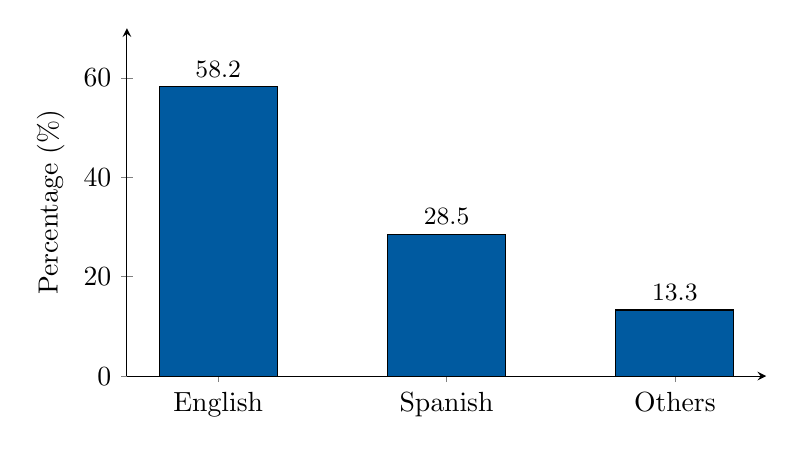
\begin{tikzpicture}
\begin{axis}[
    width=0.8\textwidth,
    height=6cm,
    ybar,
    bar width=1.5cm,
    ylabel={Percentage (\%)},
    symbolic x coords={English, Spanish, Others},
    xtick=data,
    nodes near coords,
    nodes near coords align={vertical},
    ymin=0,
    ymax=70,
    axis lines=left,
    enlarge x limits=0.2,
    legend style={at={(0.5,-0.2)}, anchor=north, legend columns=-1},
    every node near coord/.append style={font=\small}
]
\addplot[fill=darkblue] coordinates {(English, 58.2) (Spanish, 28.5) (Others, 13.3)};
\end{axis}
\end{tikzpicture}
\caption{Language distribution in the dataset (determined using Whisper large-v3)}
\label{fig:language-dist}
\end{figure}

The "Others" category encompasses content distributed across 18 different languages, highlighting the multilingual nature of our dataset and the importance of utilizing STT models with robust cross-lingual capabilities.

\section{Audio Source Separation Methods}
This study evaluates two prominent open-source audio source separation frameworks: Spleeter and Demucs. All evaluations were conducted on standardized hardware: a 40GB SMX4 A100 GPU with 6 AMD EPYC 7543 cores and 24GB of RAM.

\subsection{Spleeter}
Spleeter provides three model variants (2stems, 4stems, and 5stems) with two frequency configurations: standard (11kHz frequency cutoff) and extended (16kHz frequency range).

\begin{table}[ht]
\centering
\caption{Spleeter Performance Metrics}
\label{tab:spleeter-metrics}
\begin{tabular}{lcc}
\toprule
\textbf{Configuration} & \textbf{Processing Time (s)} & \textbf{Realtime Ratio} \\
\midrule
2stem 11kHz & 0.19 & $\sim$1148x \\
2stem 16kHz & 0.21 & $\sim$1039x \\
\bottomrule
\end{tabular}
\end{table}

As shown in Table~\ref{tab:spleeter-metrics}, Spleeter demonstrates impressive processing speeds across all configurations, making it highly efficient for large-scale deployments.

\subsection{Demucs}
We focus on the latest Hybrid Transformer Demucs generation, which offers three model variants: htdemucs (base model), htdemucs\_ft (finetuned version), and htdemucs\_6s (extended version with piano and guitar source separation).

\begin{table}[ht]
\centering
\caption{Demucs Performance Metrics}
\label{tab:demucs-metrics}
\begin{tabular}{lcc}
\toprule
\textbf{Model Variant} & \textbf{Processing Time (s)} & \textbf{Realtime Ratio} \\
\midrule
htdemucs & 4.43 & $\sim$49x \\
htdemucs\_ft & 20.14 & $\sim$11x \\
\bottomrule
\end{tabular}
\end{table}

While Demucs offers superior separation quality, particularly for complex audio mixes, this comes at the cost of significantly increased processing time compared to Spleeter, as illustrated in Table~\ref{tab:demucs-metrics}.

\section{Speech-to-Text Models}
The research focuses on multilingual, open-weights STT models, evaluating them on a test set containing five versions of each song (one unprocessed and four pre-processed versions).

\subsection{Whisper Models}
We evaluate multiple variants of OpenAI's Whisper models across different implementations, as shown in Table \ref{tab:whisper-implementations}.

\begin{table}[h]
\centering
\caption{Whisper Model Implementation Availability}
\label{tab:whisper-implementations}
\begin{tabular}{@{}lcccc@{}}
\toprule
\textbf{Model} & \textbf{OpenAI} & \textbf{HF} & \textbf{Faster} & \textbf{WhisperX} \\
& \textbf{Implementation} & \textbf{Transformers} & \textbf{Whisper} & \\
\midrule
Whisper Large v2 & \checkmark & \checkmark & \checkmark & \checkmark \\
Whisper Large v3 & \checkmark & \checkmark & \checkmark & \checkmark \\
Whisper Large v3 Turbo & \checkmark & \checkmark & \checkmark & \checkmark \\
Whisper Large v3 Turbo (FP8) & \checkmark & \checkmark & \checkmark & \checkmark \\
CrisperWhisper & $\times$ & \checkmark & \checkmark & \checkmark \\
lite-whisper-large-v3 & $\times$ & \checkmark & $\times$ & $\times$ \\
lite-whisper-large-v3-acc & $\times$ & \checkmark & $\times$ & $\times$ \\
\bottomrule
\end{tabular}
\end{table}

\subsection{NVIDIA Canary Models}
NVIDIA's contribution to multilingual STT includes two models: Canary 1B and Canary 1B Flash. These models are currently accessible exclusively through NVIDIA's NeMo Framework and support four languages (English, Spanish, German, and French).

\end{document} 